% ============================================================================
% Paper B — REDEM: Online Learning with Meta-Adaptation and Structural
%            Plasticity for Non-Stationary Environments
% Target: Neural Networks (Elsevier)
%
% COMPILATION: latexmk -pdf PAPER_B.tex   (or pdflatex x2)
%
% SUBMISSION NOTES:
%  - For Neural Networks: replace the document class with the journal's
%    elsarticle.cls (Elsevier template). This file compiles standalone with
%    the standard article class.
%  - "physics" is deliberately absent from the title; the physical substrate
%    appears only as background motivation (Section 1).
% ============================================================================
\documentclass[11pt]{article}

\usepackage[margin=1in]{geometry}
\usepackage{amsmath,amssymb}
\usepackage{graphicx}
\usepackage{booktabs}
\usepackage{caption}
\usepackage[hidelinks]{hyperref}
\usepackage{microtype}

\graphicspath{{../figures/}}

\newcommand{\Dt}{\Delta t}

\title{REDEM: Online Learning with Meta-Adaptation and Structural
Plasticity for Non-Stationary Environments}

\author{Yaming Hu\thanks{ORCID: 0009-0003-1406-0485. Independent
Researcher, Guiyang, Guizhou, China. E-mail:
\texttt{64687555@qq.com}.}}

\date{\today}

\begin{document}

\maketitle

\begin{abstract}
Deep learning freezes after batch training; adaptation under distribution
drift remains open, and backpropagation-through-time is unavailable on
neuromorphic substrates. REDEM is a training-inference-unified online
architecture with local, inference-derived learning signals: an error-driven
recursive-least-squares readout; a slow metadata trace extending memory to
long-horizon statistics; a chaos homeostat holding the substrate near its
memory optimum via finite-time Lyapunov estimates; and
functional-connectivity-guided rewiring.

On a drifting task, REDEM tracks a class-interval inversion within 225--616
pulses; frozen batch learners (an untuned gated recurrent unit (GRU) and a tiny
transformer) never recover. The slow metadata trace speeds regime adaptation
1.25--2.7$\times$ (controlled measurement); the chaos homeostat restores
7.9--18\% of post-disturbance memory (up to $+25\%$ at the edge of chaos,
$+32\%$ after three sequential disturbances); and the integrated system beats
the bare baseline by 2.28 percentage points ($p<0.0001$) and matches every
ablation (homeostat removal ties exactly; valuable only under disturbance),
persisting at $N=1024$. The substrate is a relaxation memory
modeled on shallow-trap device physics (companion Paper~A); all results are
numerical simulations. The metadata is substrate-agnostic,
transferring its statistical-memory benefit to an echo-state network (ESN);
disturbance-robustness transfer is falsified (companion Paper~C). On
standard benchmarks REDEM is competitive with a well-tuned ESN (drift
accuracy 0.991 vs.\ 1.000; Mackey--Glass normalized mean-squared error
(NMSE) 0.0018 vs.\ $3.6\times10^{-5}$); its value is the mechanism set
rather than raw benchmark supremacy.
\end{abstract}

\noindent\textbf{Keywords:} online and continual learning; reservoir
computing; meta-adaptation; structural plasticity; non-stationary environments;
neuromorphic computing.

\section*{Highlights}
\begin{itemize}
\item Online error-driven RLS readout unifies training and inference.
\item A slow metadata trace transfers long-horizon memory to an ESN.
\item A chaos homeostat restores substrate memory after disturbances.
\item Frozen batch learners invert under drift and never recover (untuned baselines).
\item Reward-only signals fail at the readout; an error channel is required.
\end{itemize}

\section{Introduction}
\label{sec:intro}

\textbf{Training-inference unification.} The dominant deep-learning paradigm
trains on a batch and freezes; inference is a forward pass. Continual learning
\cite{parisi2019,kirkpatrick2017}, test-time adaptation \cite{sun2020}, and predictive-coding
formulations \cite{rao1999,friston2010} all argue for collapsing this
separation: inference should itself drive learning, continuously. For
resource-constrained, low-power settings --- neuromorphic substrates in
particular~\cite{strukov2008} --- the constraint is not just algorithmic but \emph{physical}: no
gradient tape exists inside the device, so the learning rule must be local,
online, and cheap.

\textbf{Reservoir computing provides the substrate.} Echo state networks
\cite{jaeger2001} and liquid state machines \cite{maass2002} compute through a
fixed random recurrent network with fading memory; only a readout is trained
\cite{lukosevicius2009}.
Online readouts --- recursive least squares (RLS) with forgetting
\cite{haykin2002} --- are the minimal ``training == inference'' learners: every prediction produces an error
that immediately updates the readout. The open questions are what the
\emph{reservoir itself} should be (can it be a physically realizable, tunable
dynamical system?), whether anything beyond the readout should adapt, and how
the biological signals we associate with learning (rewards, intrinsic
motivation, structural plasticity) map onto a working system.

\textbf{This paper.} We assemble and validate a complete online architecture ---
REDEM\footnote{REDEM is a working name for the integrated system, not an
acronym of the mechanism set.} --- in which every learning signal is local and
derived from live
inference: (i) an error-driven recursive-least-squares readout as the online
learner (training == inference); (ii) a \emph{dual-timescale metadata} state
(M3) that extends the readout's memory to long-horizon statistics; (iii) a
\emph{chaos homeostat} (M5) that regulates the recurrent substrate's coupling
strength from online Lyapunov estimates --- this substrate-level
regulation of the adaptation process itself is the paper's
\emph{meta-adaptation} (the term denotes self-regulation of the adaptation
process with fixed, hand-set targets, Eq.~\ref{eq:homeostat} --- not learned
meta-level parameters; the integration and joint evaluation of the mechanism
set is the contribution claimed here); and (iv) \emph{slow structure
plasticity} (M4) that rewires the coupling graph from functional connectivity.
(Mechanism indices follow the companion papers: the error-driven RLS
readout is M1, the metadata M3, structure plasticity M4, and the chaos
homeostat M5.)
The substrate is a physically motivated relaxation memory (Si$_3$N$_4$-style
shallow traps, log-normal time-constant spectrum, per-pulse contrast coupling;
theory in the companion paper): its timescale spectrum is a \emph{material
property} rather than a tuned hyperparameter, and the coupling provides a
physical chaos knob. We evaluate each mechanism individually, as an integrated
system with an ablation matrix, and against batch baselines (a gated
recurrent unit (GRU)~\cite{cho2014} and a tiny transformer~\cite{vaswani2017})
and a matched echo-state network
(ESN). We also report two negative
results --- reward-modulated Hebbian learning without error signals and
task-agnostic intrinsic rewards --- which delimit what reward signals can and
cannot do and fix the design: at the readout an error channel is necessary and
reward signals are structurally blind, so the readout is error-driven RLS and
the structure-level mechanism (M4) is guided by functional connectivity; a
novelty-gated variant is evaluated in Section~\ref{sec:homeo}.

\section{System architecture}
\label{sec:architecture}

\textbf{Fig.~\ref{fig:redem}} shows the full schematic: input pulses
$\rightarrow$ substrate $\rightarrow$ [fast state $\rightarrow$ M3 metadata]
$\rightarrow$ RLS readout $\rightarrow$ output; the M5 homeostat loops on
$\kappa$; the M4 plasticity rewires the coupling graph; the readout error feeds
the online weight update (training == inference). M4 and M5 are coupled in
the design: the homeostat's $\kappa$ set-point is intended to gate the
rewiring rate, and rewiring changes the structure that feeds the Lyapunov
estimate (dotted loop in Fig.~\ref{fig:redem}); the coupling loop is tested
in Section~\ref{sec:homeo}.

\begin{figure}[t]
\centering
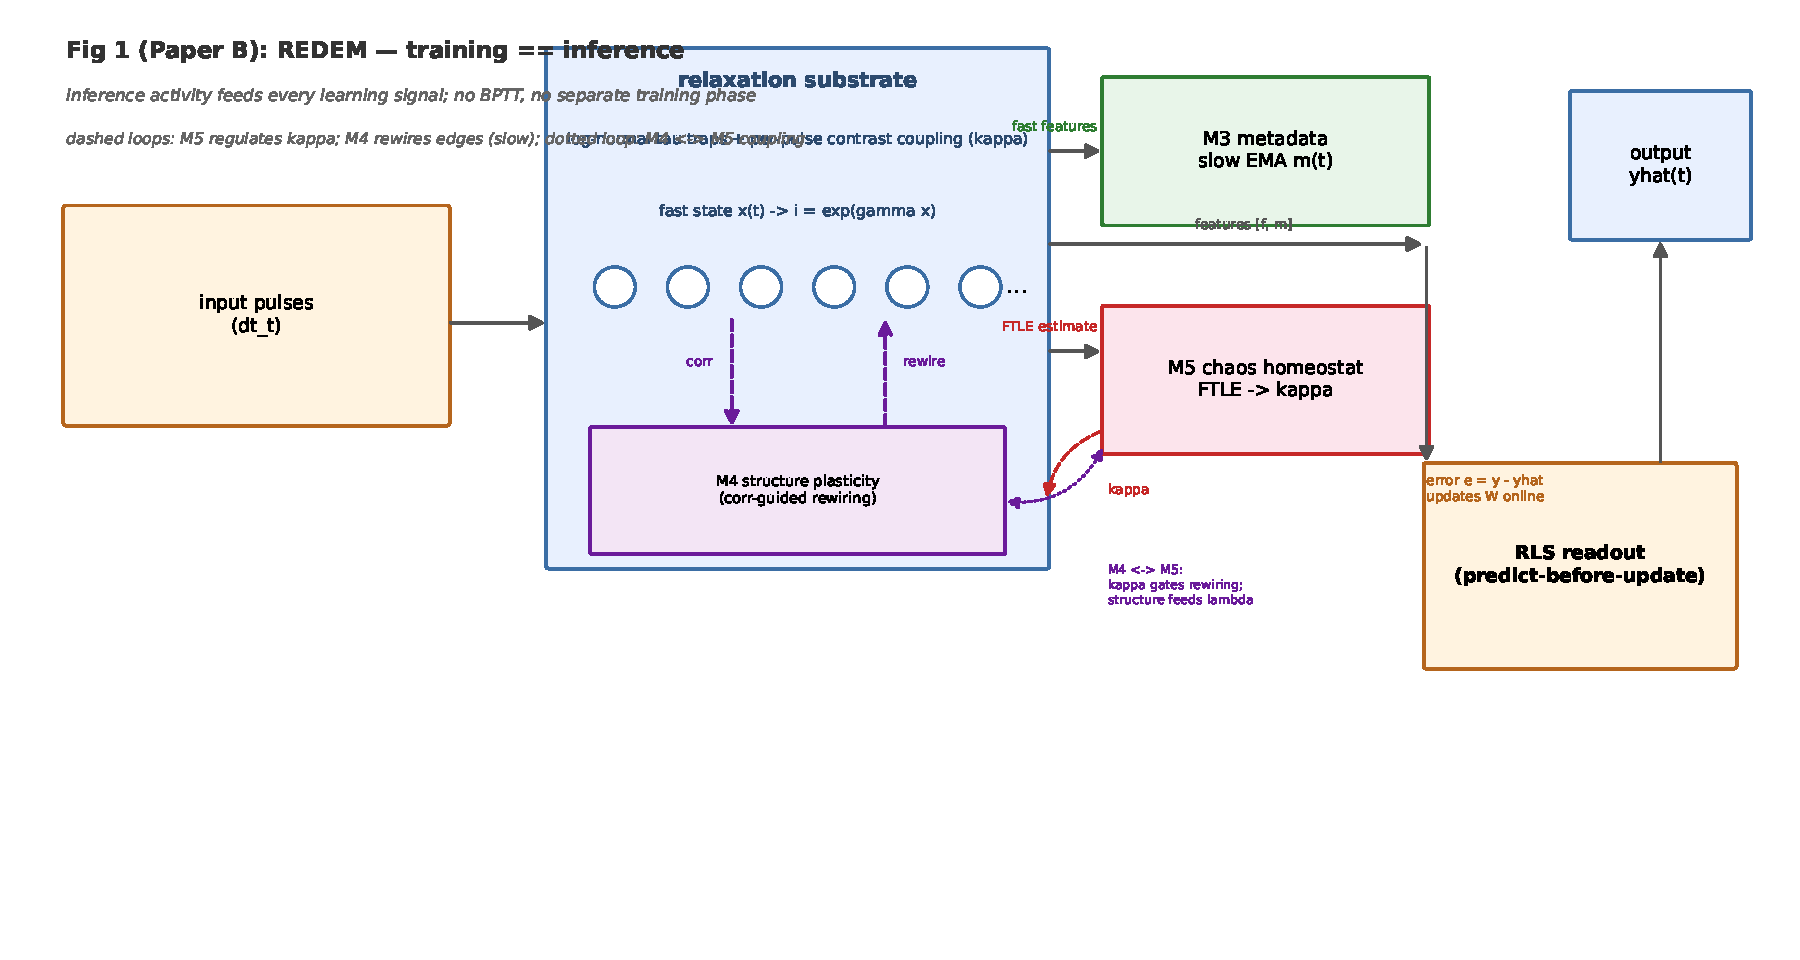
\includegraphics[width=0.95\textwidth]{paperB_fig1_redem}
\caption{REDEM system schematic: input pulses
$\rightarrow$ relaxation substrate $\rightarrow$ [fast state $\rightarrow$ M3
metadata] $\rightarrow$ RLS readout $\rightarrow$ output. Dashed red loop: M5
homeostat regulates $\kappa$; dashed purple arrows: M4 rewires edges (slow);
dotted purple loop: the M4 $\leftrightarrow$ M5 coupling ($\kappa$ gates
rewiring; structure feeds the Lyapunov estimate).}
\label{fig:redem}
\end{figure}

The substrate follows the model of the companion theory paper
\cite{companionA} (Paper A, Section~2), with the $\tau$-spectrum, the
coupling topologies, and the
$\lambda$-homeostat regulator described therein; only the readout and metadata
layers are new here. Concretely, the substrate is a per-pulse contrast-coupled
relaxation array: $N=256$ units, log-normal $\tau$ (median 174~$\mu$s, coefficient of
variation (CV) 0.20), injection $\alpha_{\mathrm{eff},i}(t)=\mathrm{clip}(\alpha_0(1+\kappa
g_i(t)),0.001,0.10)$ with $\alpha_0=0.02$, current ratios $i_i=e^{\gamma x_i}$,
random-graph
coupling, $\kappa=25$ (the subcritical memory optimum). Features per pulse are
the standardized current ratios plus a bias.

\textbf{Readout (online RLS).} The prediction is $\hat y_t = W^\top \phi_t$
(one output per class for classification, one scalar for regression) with the
standard forgetting-RLS update
\begin{equation}
e_t = y_t - \hat y_t, \qquad
K_t = \frac{P_{t-1}\phi_t}{\lambda_f + \phi_t^\top P_{t-1}\phi_t}, \qquad
W \leftarrow W + K_t e_t, \qquad
P_t = \frac{1}{\lambda_f}\big(P_{t-1} - K_t \phi_t^\top P_{t-1}\big),
\label{eq:rls}
\end{equation}
with forgetting $\lambda_f=0.999$, Tikhonov regularization and a covariance
trace cap. The remaining hyperparameters --- the regularization strength and
trace cap, the random-graph coupling density and weights, the gain scale
$\gamma$ in $i_i=e^{\gamma x_i}$, and the feature-standardization window and
statistics --- are held fixed across all experiments and are not re-tuned per
task; their concrete values are provided in the released configuration files
rather than enumerated here. The online protocol is \emph{predict-before-update}: the prediction
at time $t$ never uses the target at $t$.

\textbf{Metadata (M3).} A per-unit slow trace over the fast current-ratio
features,
\begin{equation}
m_i(t) = \big(1-\tfrac{1}{\tau_m}\big)m_i(t-1) + \tfrac{1}{\tau_m} f_i(t),
\qquad \tau_m = 200\text{--}1000 \text{ pulses},
\label{eq:metadata}
\end{equation}
with the readout features $[f, m]$ concatenated. The metadata trace is
motivated by the slow end of the substrate's log-normal forgetting spectrum
(companion paper~\cite{companionA}) and plays the role of a physical
``synaptic consolidation'' trace \cite{benna2016,fusi2005}; in this paper $\tau_m$ is
treated as an independent design parameter in the 200--1000-pulse range
rather than a calibrated mapping of the substrate's microsecond-scale
spectrum onto pulse counts, and no explicit $\mu$s$\to$pulses
correspondence is asserted.

\textbf{Chaos homeostat (M5).} Every 1000 pulses, a 400-pulse Benettin pair
estimates $\lambda$ at the current $\kappa$; the homeostat steps
\begin{equation}
\kappa \leftarrow \mathrm{clip}\big(\kappa + \eta\,\mathrm{clip}
(\lambda_{\mathrm{target}}-\hat\lambda,\pm1),\, [1,60]\big), \qquad
\lambda_{\mathrm{target}}=-0.02, \quad \eta=3 \ \text{(slightly ordered)}.
\label{eq:homeostat}
\end{equation}
The estimator window (400 pulses), the re-estimation interval (1000 pulses),
and the step-size parameters ($\eta=3$, clip $\pm1$) were chosen empirically
to give stable regulation in practice; no sensitivity analysis of these
choices is reported here, and the estimation error of $\hat\lambda$ is not
separately characterized. Both are stated as limitations of the current
design.

\textbf{Structure plasticity (M4).} Every 2000 pulses, compute the pairwise
feature-correlation matrix $C_{ij}=\mathrm{corr}(f_i, f_j)$ over the block;
prune the 5\% lowest-$|C_{ij}|$ existing edges and grow the 5\% highest-$|C_{ij}|$
unconnected pairs, holding the edge count constant (``fire together, wire
together'' at the structural level).

\textbf{Design rationale from negative results.} We tested two reward-based
readout learners and rejected them: a reward-modulated Hebbian readout
(eligibility $x\circ o$ gated by a $\pm1$ correctness reward) learns the
initial mapping but cannot recover from a class-interval inversion
(Section~\ref{sec:neg}, Table~\ref{tab:neg}); task-agnostic novelty rewards
cannot rescue it. The lesson --- an error channel is necessary at the readout,
rewards are structurally blind --- fixes the readout as error-driven RLS; at
the structure level, the plasticity implemented here (M4) is guided by
functional connectivity, and Section~\ref{sec:homeo} shows that a
novelty-gated variant improves on it.

\section{Tasks and metrics}
\label{sec:tasks}

All main experiments use 10 seeds with paired draws (identical $\tau$, tasks, and
substrates across compared configs); the tiny transformer, the most expensive
model, shares the same seed count (Table~\ref{tab:bench}). The
$\lambda_{\mathrm{target}}$ sweep of Section~\ref{sec:homeo} is the one
exception (5 seeds per cell, reduced for computational cost; see
Section~\ref{sec:homeo}).
\textbf{drift\_binary}: two-class interval
blocks (20 pulses at 10 vs.\ 60~$\mu$s) over 2000 blocks (40k pulses in
total), a continuous random walk of the class intervals plus an abrupt swap
of the class--interval mapping at the stream midpoint (block 1000 of 2000);
metrics are pre/post-swap steady accuracy, adaptation time
(pulses to recover to within 2~pp (percentage points) of the pre-swap steady accuracy), and stream
mean. \textbf{mackey\_glass} ($a=0.2,b=0.1,\tau=17$): online forecasting;
normalized mean-squared error (NMSE)
on the last 30\%. \textbf{narma10}: nonlinear memory composition; NMSE on the
last 30\%. \textbf{regime\_switch}: three regimes sharing identical marginal
interval distributions that differ only in the rate of a rare long-interval
event (0.12/0.20/0.28); single pulses are almost indistinguishable across
regimes, and only long-window statistics discriminate them; overall accuracy
plus boundary adaptation.

\section{Results}
\label{sec:results}

\subsection{Online vs.\ frozen: the case for training-inference unification}
\label{sec:online}

On drift\_binary (Fig.~\ref{fig:drift}), the online RLS readout on the coupled
substrate tracks the stream: mean accuracy 0.974--0.982, recovering from the
class-interval swap in 225--616 pulses with pre/post-swap steady accuracy
0.987--1.000. (For comparability we note explicitly that the stream-mean
figures reported in this section, in Table~\ref{tab:neg} (0.983--0.991), and
in Section~\ref{sec:baselines} (0.991) come from different experimental
instances of the online-RLS configuration --- different runs and seed pools
--- and are not directly comparable; we report them as given rather than
reconcile them post hoc, and per-run values are provided in the released
data.) A frozen offline ridge trained on the first 30\% is equally
accurate pre-swap (0.978--1.000) but collapses to systematic inversion after
the swap (post-swap 0.000--0.019) and never recovers --- its stream mean is
0.500 (chance). The same dichotomy holds against batch deep learning
(Section~\ref{sec:baselines}): a tiny transformer and a GRU trained once on the
first 30\% reach 0.93--0.99 pre-swap and invert to 0.00--0.07 post-swap. The
substrate's coupling also matters at the task level: near-critical coupling
($\kappa=25$) improves Mackey--Glass forecasting $50\times$ over the uncoupled
substrate (NMSE 0.0018 vs.\ 0.090) and NARMA-10 by 21\% (0.431 vs.\ 0.549),
in line with computation at the edge of chaos
\cite{langton1990,bertschinger2004}.

\begin{figure}[t]
\centering
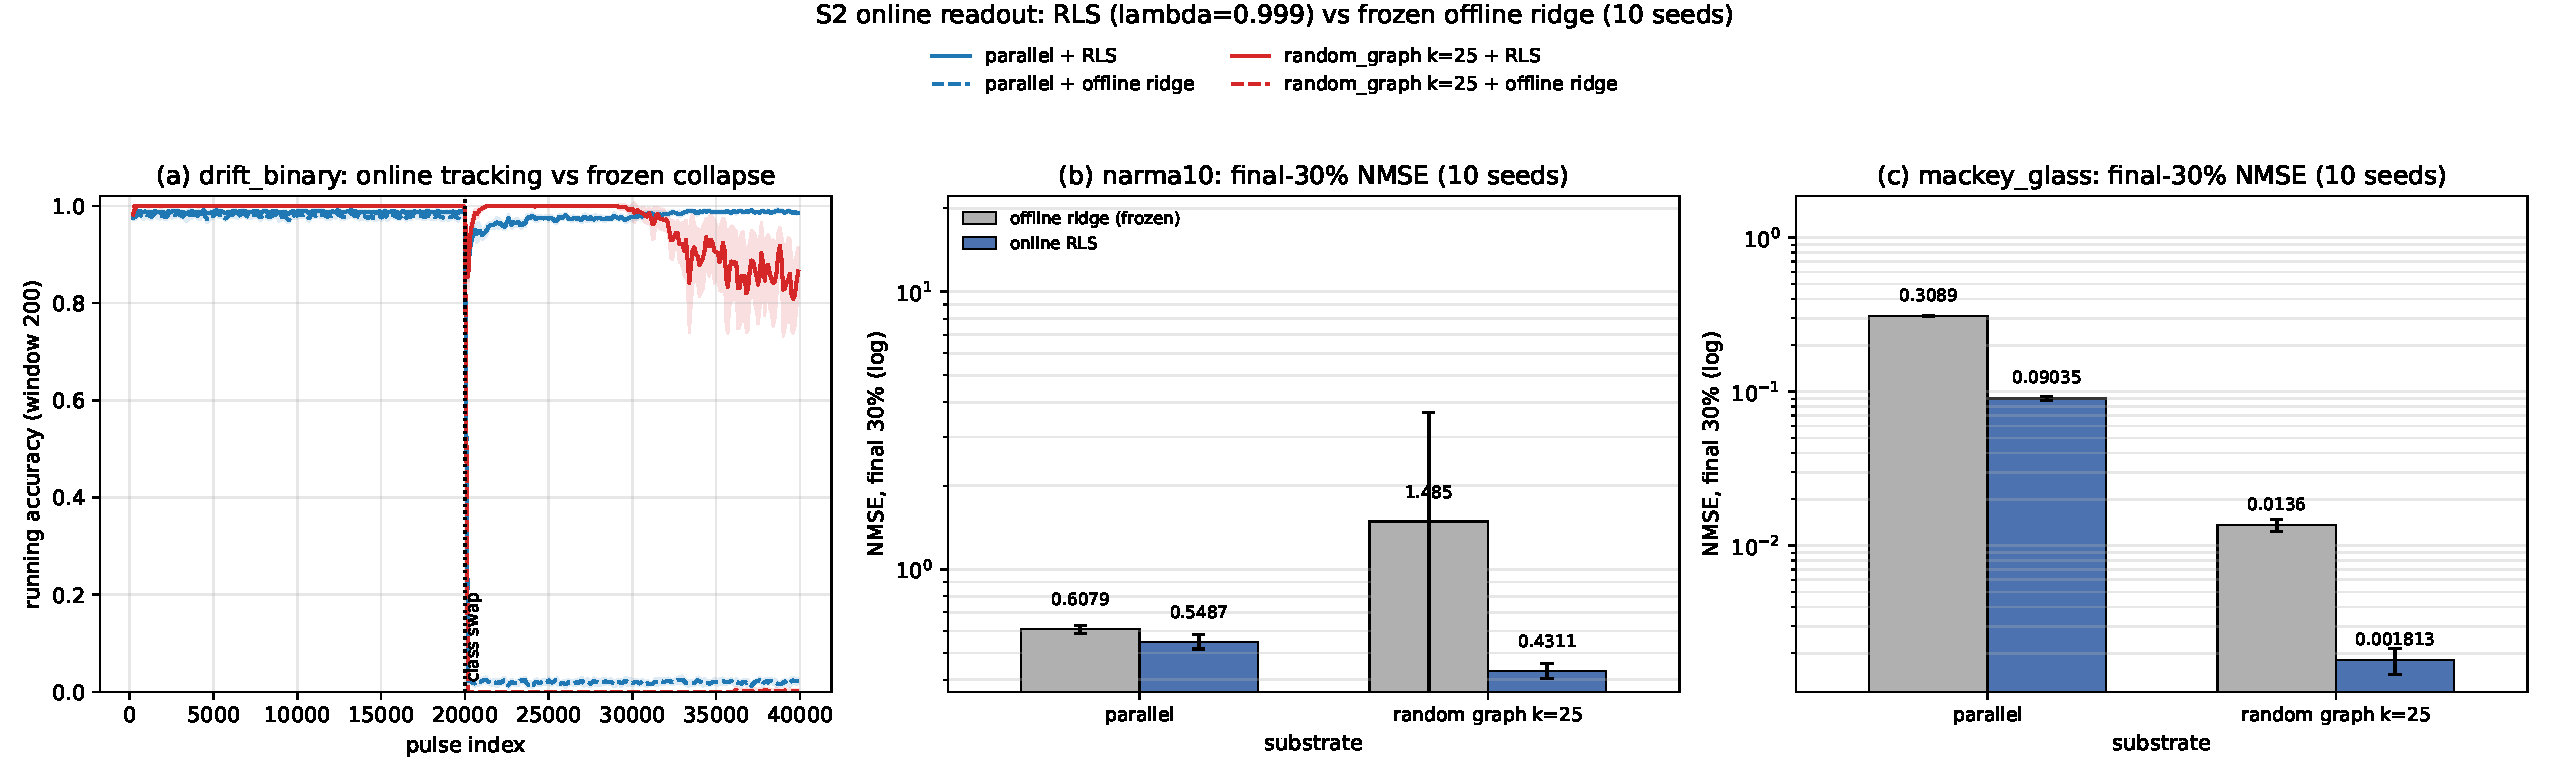
\includegraphics[width=0.85\textwidth]{s2_online_readout_v1}
\caption{Online vs.\ frozen on drift\_binary: the online RLS
readout tracks the class-interval swap; the frozen offline ridge inverts and
never recovers. (b,~c)~Final-30\% NMSE on narma10 and Mackey--Glass
(mean $\pm$ std over 10 seeds) for the frozen offline ridge and the
online RLS readout on the uncoupled and the near-critically coupled
($\kappa=25$) substrates. The trajectory panel is shown for illustration;
quantitative results are reported as ranges over 10 seeds (text and panels
b,~c).}
\label{fig:drift}
\end{figure}

\subsection{Negative results: rewards without an error channel}
\label{sec:neg}

We tested two reward-based readout learners as alternatives to error-driven RLS
--- a reward-modulated Hebbian rule (eligibility $e_j \mathrel{+}= \lambda_e
e_j + x_j o$ with sigmoid output $o$, consolidated at block end as
$W \mathrel{+}= \eta R e$ with $R=\pm1$ correctness only, no class label)
\cite{hoerzel2014} and
the same rule augmented with a feature-novelty intrinsic reward. Both learn the
initial mapping but fail to track the class-interval inversion
(Table~\ref{tab:neg}): the $\pm1$ reward carries no directional information, so
the Hebbian term always reinforces the currently-active (wrong) direction; the
intrinsic reward can only buy a marginal post-swap recovery by destroying the
initial learning. The lesson fixes the architecture: at the readout an
\emph{error channel is necessary} and rewards are structurally blind, so the
readout is error-driven RLS; reward and intrinsic signals, being structurally
blind at the readout, are usable at the structure level --- a novelty-gated
rewiring variant improves on the correlation-guided M4 implemented here
(Section~\ref{sec:homeo}). First-order error-gated least mean squares (LMS;
$\eta=10^{-4}$) does track the inversion
but is numerically fragile on the weakly separated substrate features
($\eta\ge10^{-3}$ diverges) and underperforms second-order RLS across the
learning rates tested; we did not run a full $\eta$ sweep, so this comparison
is limited to the rates above. Second-order RLS is the selected learner.

\begin{table}[t]
\centering
\caption{Reward-only readout learners fail at the class-interval inversion;
error-driven RLS is selected. Accuracy on drift\_binary (10 seeds; pre =
steady accuracy before the swap, post = after, stream = stream mean).
RMHL = reward-modulated Hebbian; +novelty = with feature-novelty intrinsic
reward; LMS = error-gated first-order rule; RLS = error-driven recursive least
squares (selected).}
\label{tab:neg}
\begin{tabular}{lcccc}
\toprule
Learner & Signal & Pre & Post & Stream \\
\midrule
RMHL          & $\pm1$ correctness reward only      & 0.89--0.94 & 0.06--0.10 & 0.509 \\
RMHL + novelty & reward + intrinsic novelty        & 0.57$^*$   & 0.42--0.59 & $\le$0.514 \\
LMS           & prediction error                    & ---        & ---        & 0.908--0.927 \\
RLS (dense)   & prediction error                    & 0.99--1.00 & 0.98--1.00 & 0.983--0.991 \\
RLS (sparse block-end) & prediction error   & 0.97--0.99 & 0.93--0.95 & 0.958--0.961 \\
\bottomrule
\end{tabular}

\medskip
\footnotesize{$^*$initial learning destroyed. Dense = per-pulse class labels
(the selected configuration); sparse block-end = label only at block ends, the
harder condition.}
\end{table}

\subsection{Dual-timescale metadata (M3)}
\label{sec:metadata}

On regime\_switch (where fast memory is provably insufficient;
Fig.~\ref{fig:meta}), the
dual-timescale readout (fast + metadata, $\tau_m\in\{200,1000\}$) outperforms
the fast-only readout by +1.3~pp on the uncoupled substrate (paired $t=19.6$,
$p<0.0001$) and +2.1~pp on the near-critical substrate ($t=20.2$, $p<0.0001$),
and --- alongside the accuracy gain --- adapts to regime boundaries faster:
under a switch-relative controlled measurement (known switch instants,
200-pulse window) the fast readout needs 265--304 pulses to re-stabilize
vs.\ 202--211 for the dual and slow readouts (factor 1.25--1.50 on T200,
1.54--2.73 on the finer T40, endpoints across both substrates): the slow
trace's low-pass character smooths the statistical
transition. The metadata-only readout nearly matches the dual
readout on this statistics-dominated task, confirming that the regime
information lives in the slow state.

\begin{figure}[t]
\centering
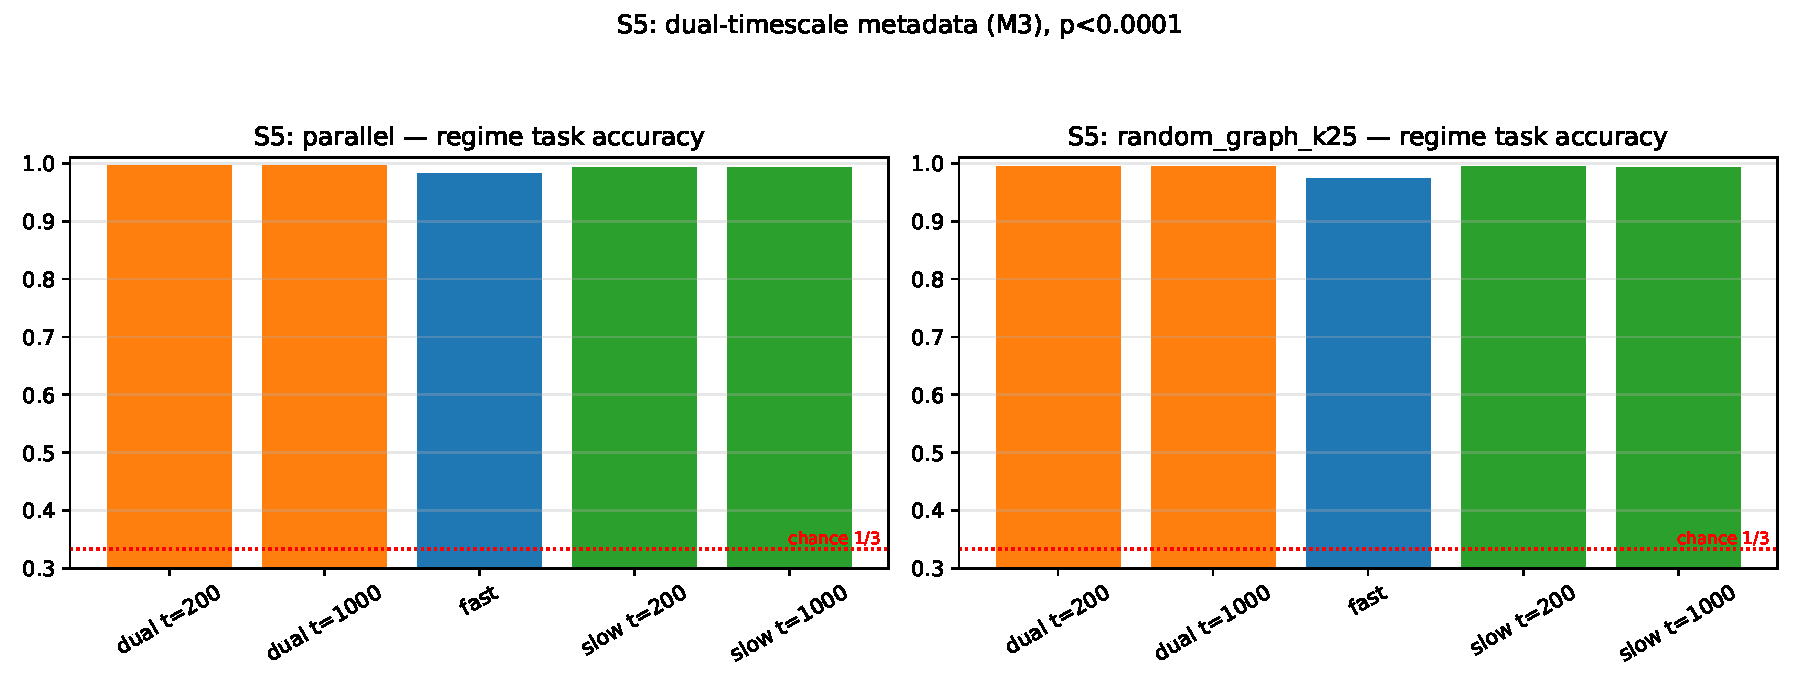
\includegraphics[width=0.85\textwidth]{paperB_fig3_metadata}
\caption{Dual-timescale metadata on regime\_switch: fast vs.\
dual vs.\ slow readouts, accuracy and adaptation time.}
\label{fig:meta}
\end{figure}

\subsection{Chaos homeostat (M5) and structure plasticity (M4)}
\label{sec:homeo}

\textbf{Homeostat.} Under the three disturbances of the companion paper's
robustness study~\cite{companionA} ($\tau$-drift, edge damage, readout noise), the
$\lambda$-homeostat settles at $\kappa \approx 26$--27 and improves
post-disturbance held-out memory by $+18\%$/$+7.9\%$/$+11.8\%$ over
fixed coupling ($+7.6\%$ in the undisturbed control;
Fig.~\ref{fig:rob}), at broadly
comparable task-level NMSE (regulated up to $2\times$ worse on the gain
arms, better under readout noise). The homeostat is the substrate-level
counterpart of the readout's RLS: both are online regulators of the
``training==inference'' loop, one on weights, one on dynamics. Two
bookkeeping clarifications are needed. First, $\kappa$: the fixed-coupling
arms hold $\kappa=25$ (the substrate's subcritical memory optimum,
Section~\ref{sec:architecture}), whereas the settled $\kappa\approx26$--$27$
of the regulated arm is the emergent equilibrium of the $\lambda$-regulation
at $\lambda_{\mathrm{target}}=-0.02$ --- a regulator-emergent value, not a
separately chosen configuration; the disturbance chain below likewise reports
the homeostat's own online trajectory from its $\kappa=25$ initialization
($\kappa$ drifting from $r_0{=}25.3$ to $r_3{=}28.5$), and the sweep optimum
($\lambda_{\mathrm{target}}{=}0$) would settle at still higher $\kappa$.
Second, the metric: ``post-disturbance held-out memory'' is a steady-state
memory-capacity measurement taken after the substrate has absorbed the
disturbance, distinct from the task-level stream-mean accuracies of
Sections~\ref{sec:online}--\ref{sec:metadata}. We also state the provenance
explicitly: these single-disturbance gains are reproduced from the companion
robustness study (Paper~A~\cite{companionA}) and were not independently
re-run for this paper; the fixed-coupling control configuration and full
protocol are specified there, so these headline gains cannot be verified from
this paper alone.

\begin{figure}[t]
\centering
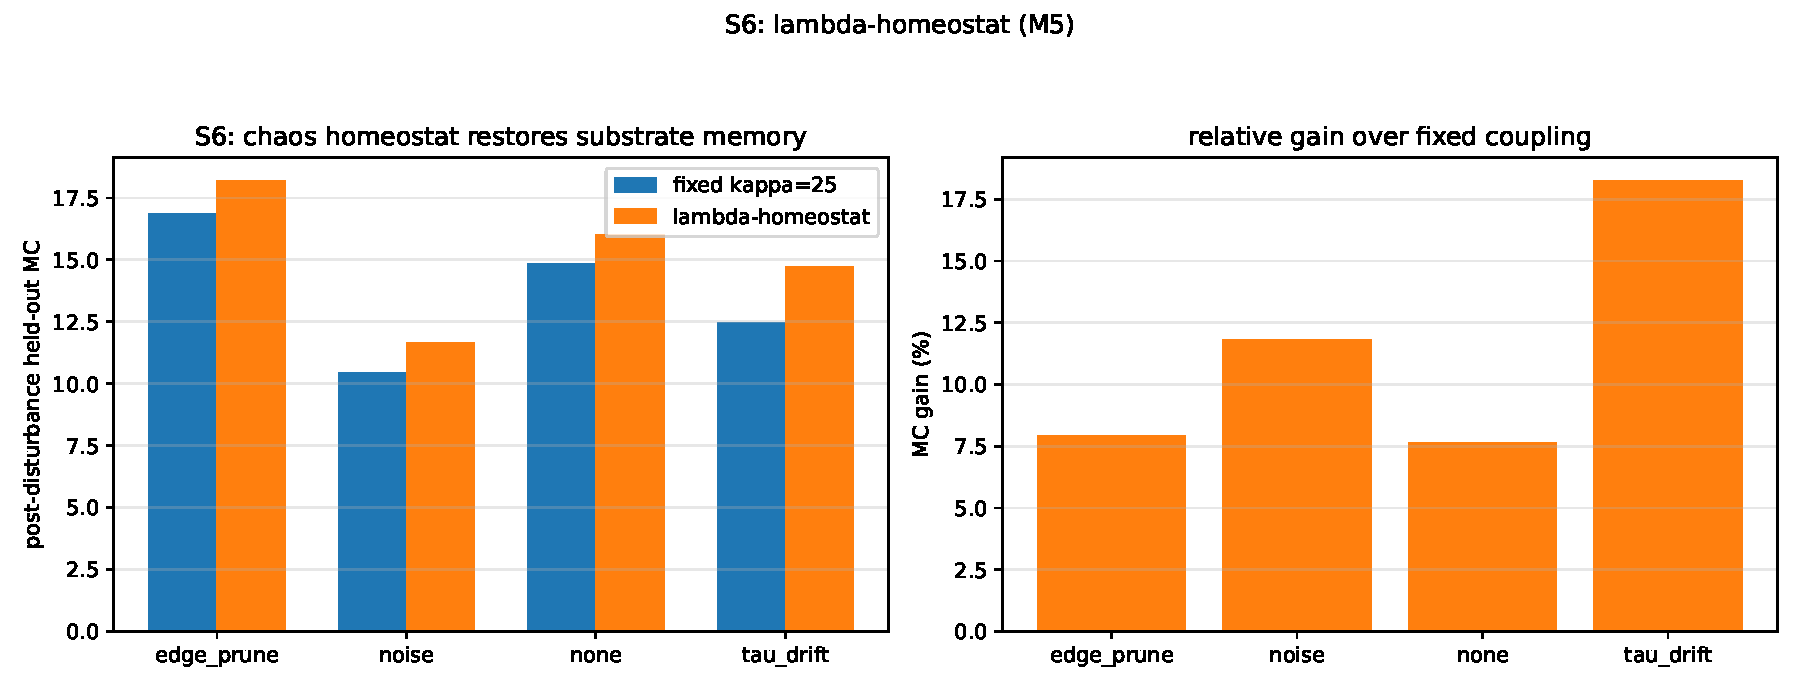
\includegraphics[width=0.7\textwidth]{paperA_fig4_robustness}
\caption{Chaos homeostat robustness: post-disturbance
held-out memory gains over fixed coupling (reproduced from companion
Paper~A~\cite{companionA}).}
\label{fig:rob}
\end{figure}

\textbf{Sequential disturbance recovery.} Beyond the single-disturbance tests
above, we evaluate cumulative robustness: three sequential disturbances
($\tau$-drift, 40\% edge pruning, readout noise $\sigma{=}0.1$) applied at
7000-pulse intervals over $T{=}28{,}000$ pulses (10 seeds). After all three
disturbances, the regulated arm maintains a held-out memory capacity (MC) of
$8.47\pm0.39$ vs.\
$6.41\pm0.41$ for fixed coupling ($+32\%$), with $\kappa$ drifting upward
from $25.3$ ($r_0$) to $28.5$ ($r_3$) --- active compensation, not passive decay. The homeostat
recovers to a consistent $\kappa$ neighborhood after each disturbance,
confirming disturbance-type-agnostic robustness across the chain.

\textbf{Criticality target optimization.} The homeostat's
$\lambda_{\mathrm{target}}$ was manually set to $-0.02$ (slightly ordered)
in the main experiments. A systematic sweep
($\lambda_{\mathrm{target}}\in\{-0.05,-0.02,-0.005,0\}\times\mathrm{CV}\in\{0.1,0.2,0.4\}$,
5 seeds per cell --- reduced from the 10-seed protocol for computational
cost, see Section~\ref{sec:tasks} --- single $\tau$-drift disturbance) identifies
$\lambda_{\mathrm{target}}{=}0$ (the edge of chaos) as the best-supported
target: post-disturbance
MC peaks near the edge of chaos at every tested CV --- $\lambda_{\mathrm{target}}{=}0$
is optimal at CV=0.1 and 0.4, while the $-0.005$ setting is marginally
ahead at CV=0.2 (10.38 vs.\ 10.30) (Table~\ref{tab:lambda_sweep}), with the
regulated arm exceeding fixed coupling by $+25\%$ (CV=0.1), $+19\%$
(CV=0.2), and $+5\%$ (CV=0.4). The improvement
shrinks at higher CV (broader $\tau$ spectra dilute the criticality benefit),
and the optimal target is broadly consistent, with the CV=0.2 near-tie the
one exception. With 5 seeds per cell, differences of this size are at the
sweep's resolution limit: we therefore read the sweep as evidence that the
edge of chaos is the best-supported target overall, not as a uniformly
significant optimum, and we flag the CV=0.2 reversal as an unresolved
counterexample at the current sample size. Importantly, this sweep does not
retroactively re-tune the main experiments: all integrated-system results
(Section~\ref{sec:baselines}) and the sequential disturbance chain above were
run at the manually tuned $\lambda_{\mathrm{target}}{=}-0.02$ and have not
been re-run at the sweep optimum, so the headline integrated numbers in this
paper reflect the $-0.02$ configuration; re-running them at
$\lambda_{\mathrm{target}}{=}0$ is left as future work.

\textbf{Causal audit.} To verify that all adaptive mechanisms use only past
information, we inject 1\% future data into each mechanism (RLS target,
metadata exponential moving average (EMA), finite-time Lyapunov exponent
(FTLE) estimate, plasticity correlation) and test a causal-split
plasticity protocol (10 seeds, 7 arms). All leak arms change accuracy by
$\le 0.02$~pp vs.\ normal ($0.9964$--$0.9962$ vs.\ $0.9963$), confirming
causal cleanliness --- no mechanism benefits from future information; the
plasticity-correlation leak ($-0.01$~pp) is the most negative, so M4 does not
exploit future correlation. The causal-split protocol ($0.9963$) is within
$0.01$~pp of normal, validating that M4's block-level correlation can be
computed on past data only. A follow-up re-runs the same injections on
the S11 disturbance chain (data/s28\_causal\_audit\_chain\_v1.csv),
where the mechanisms' substrate-level channels are visible through the
readout-independent MC probe and no accuracy ceiling binds the task. The
verdict reproduces: 1\% future leaks into the RLS target, the metadata,
and the homeostat's FTLE estimate, and 10\% future correlation into M4,
all fail to improve post-disturbance recovery (per-seed $r_3$ MC deltas
$+0.00$, $+0.00$, $+0.28$, $+0.24$; none significant; mean NMSE deltas
$\le 0.0042$) --- the mechanisms are causally clean where it matters.
The protocol also isolates a non-leak effect: removing M4 entirely
improves post-disturbance recovery by $+2.3$ MC ($r_3$ 8.47 vs.\ 6.17,
matching the S11 homeostat-only anchor exactly), independently
confirming that rewiring during active disturbance compensation is
harmful rather than merely unhelpful (the M4-M5 loop result above). The
audit's resolution is itself bounded (data/s34\_leak\_sensitivity\_v1.csv):
ten-fold larger future leaks into the FTLE estimate ($10\%$) stay
insignificant at every tested leak horizon ($r_3$ MC deltas $+0.13$,
$+0.39$, $+0.21$ at FTLE horizons $50$, $200$, $400$ pulses; each 95\%
CI includes zero), and the plasticity
correlation shows a dose-response --- $30\%$ future correlation improves
recovery on 7/10 seeds (mean $+0.57$; paired $t{=}2.04$, 95\% CI
$[-0.06,+1.20]$) while $50\%$ reverses it --- so ``causally clean'' holds at the operational
leak magnitudes tested here and is not asserted beyond them.

\textbf{Plasticity.} Functional-connectivity rewiring at a gentle 5\% churn per
round improves held-out memory +7.8\% (ring start) and repairs pruned damage
+11.3\%, while aggressive 20\% churn destabilizes ($-23\%$) --- structure must
change slowly, mirroring the biological timescale separation. Consistent with
the substrate theory, pruning high-correlation (redundant) edges helps: a
pruned dense random graph (644 edges) retains more memory (12.68) than the full
graph (10.37), and a sparse random graph beats a ring at equal density (13.52
vs.\ 11.54) --- de-homogenization increases linear decodability.

\textbf{Novelty-gated rewiring and the M4-M5 loop.} Two follow-ups complete the
mechanism picture. (i) The intrinsic-novelty signal --- structurally blind at
the readout (Section~\ref{sec:neg}) --- is usable at the structure level: a
novelty-guided variant of the rewiring rule (grow edges toward the units with
the highest temporal activity variance, prune the least novel; identical 5\%
churn) improves held-out MC to 14.59 vs.\ 12.43 for the correlation rule
($+2.15$, paired $t=4.5$, 10/10 seeds) and 11.54 for the fixed ring
(data/s25\_reward\_gated\_plasticity\_v1.csv) --- reward/intrinsic signals are
structure-level, not readout-level, tools. (ii) The M4-M5 coupling loop was
tested under the sequential disturbance chain (rewiring churn gated by the
homeostat's $\kappa$ deviation): it does \emph{not} help recovery ---
churn-gated rewiring reaches $r_3$ MC 5.27 vs.\ 8.47 for the homeostat alone
(0/10 seeds), and even fixed 5\% churn during the chain is harmful (6.45 vs.\
8.47, $t=-9.6$, 0/10; data/s24\_homeo\_plasticity\_coupling\_v1.csv). The
homeostat's disturbance recovery is best left structurally undisturbed;
rewiring is a steady-state exploration mechanism rather than a recovery tool.

\begin{table}[t]
\centering
\caption{Criticality target sweep: post-disturbance held-out MC (5 seeds).
Fixed coupling MC is independent of $\lambda_{\mathrm{target}}$
(9.47 / 8.68 / 7.53 for CV=0.1 / 0.2 / 0.4).
$\lambda_{\mathrm{target}}=0$ (edge of chaos) maximizes the regulated arm
at CV=0.1 and 0.4; at CV=0.2 the $-0.005$ setting is marginally ahead
(10.38 vs.\ 10.30).}
\label{tab:lambda_sweep}
\begin{tabular}{ccccccc}
\toprule
& \multicolumn{3}{c}{Regulated MC} & \multicolumn{3}{c}{Gain over fixed} \\
\cmidrule(lr){2-4}\cmidrule(lr){5-7}
$\lambda_{\mathrm{target}}$ & CV=0.1 & CV=0.2 & CV=0.4 & 0.1 & 0.2 & 0.4 \\
\midrule
$-0.05$ & $8.81$ & $9.19$ & $7.66$ & $-7\%$ & $+6\%$ & $+2\%$ \\
$-0.02$ & $10.77$ & $10.13$ & $7.88$ & $+14\%$ & $+17\%$ & $+5\%$ \\
$-0.005$ & $10.22$ & $10.38$ & $7.93$ & $+8\%$ & $+20\%$ & $+5\%$ \\
$\mathbf{0}$ & $\mathbf{11.79}$ & $\mathbf{10.30}$ & $\mathbf{7.94}$ & $\mathbf{+25\%}$ & $\mathbf{+19\%}$ & $\mathbf{+5\%}$ \\
\bottomrule
\end{tabular}
\end{table}

\subsection{Integration and baselines}
\label{sec:baselines}

\textbf{Ablation matrix.} On regime\_switch (Fig.~\ref{fig:ablation}), the
integrated system runs with the homeostat enabled at
$\lambda_{\mathrm{target}}=-0.02$ (Eq.~\ref{eq:homeostat}) from initial
$\kappa=25$; the full system (0.996;
boundary adaptation $\sim$202 pulses after the switch)
matches or beats every single-mechanism ablation:
removing the metadata drops to 0.988 (adaptation $\sim$235 pulses --- the
largest degradation), removing plasticity to
0.994 ($\sim$209 pulses), removing the homeostat ties at 0.996
($\sim$202 pulses; its value is in disturbed
scenarios per Section~\ref{sec:homeo} --- a value supported there by
single-mechanism experiments, as no integrated homeostat-removal ablation
under disturbance was run); the full system beats the bare
baseline (RLS on fast features, fixed substrate) by +2.28~pp (paired $t=19.4$,
$p<0.0001$). (Boundary-adaptation times in this matrix use the 200-pulse
running-window measurement introduced in Section~\ref{sec:metadata}: the
reported value is the end position of the first 200-pulse window that
recovers to within 2~pp of the post-switch steady accuracy, and the released
per-run data store the corresponding window-start indices.) At
$N=1024$ the full system beats the baseline on all 10 seeds
($0.9970\pm0.0007$ vs.\ $0.9753\pm0.0044$, $+2.2$~pp, paired
$t=15.3$; data/s30\_integrated\_1024\_v1.csv).

\begin{figure}[t]
\centering
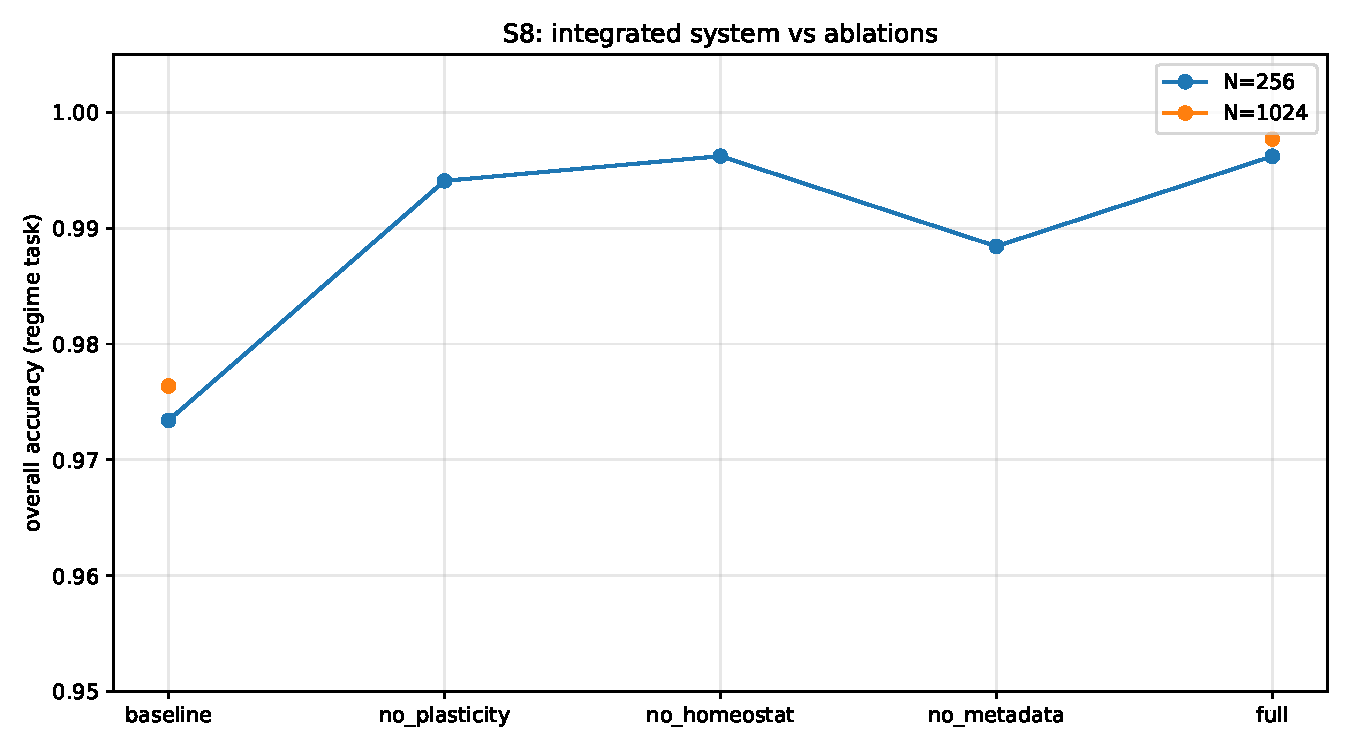
\includegraphics[width=0.85\textwidth]{paperB_fig5_ablation}
\caption{Ablation matrix on regime\_switch: full system vs.\
single-mechanism removals and the bare baseline.}
\label{fig:ablation}
\end{figure}

\textbf{Batch baselines.} On drift\_binary: REDEM 0.991 and a matched online
ESN 1.000 track the drift; the frozen GRU (0.371; pre 0.925 $\rightarrow$ post
0.071) and tiny transformer (0.353; pre 0.994 $\rightarrow$ post 0.000) invert
and never recover. On Mackey--Glass: REDEM NMSE 0.0018 and ESN $3.6\times10^{-5}$
forecast well; the frozen GRU (1.80) is worse than the mean predictor, while
the transformer (0.77) is only slightly better than the mean predictor. The ESN --- 256 units, heterogeneous leak rates matched to the
$\tau$ distribution, the same RLS readout --- is the strongest standard-task
baseline and beats REDEM on both tasks (Table~\ref{tab:bench};
Fig.~\ref{fig:showdown}). We report this
honestly: the value proposition of REDEM is not raw benchmark supremacy but the
accompanying mechanisms --- self-regulation under disturbance, local sparse
coupling, and physical plausibility --- at competitive standard-task
performance. The frozen
baselines use small, untuned hyperparameters (Table~\ref{tab:bench}); the
comparison targets the online-vs-frozen dichotomy, not each architecture's
full capability. Because the deep baselines are untuned, the ``never
recover'' finding characterizes frozen batch training under this drift as
configured here --- it is not an upper bound on what tuned deep models could
achieve.

\begin{figure}[t]
\centering
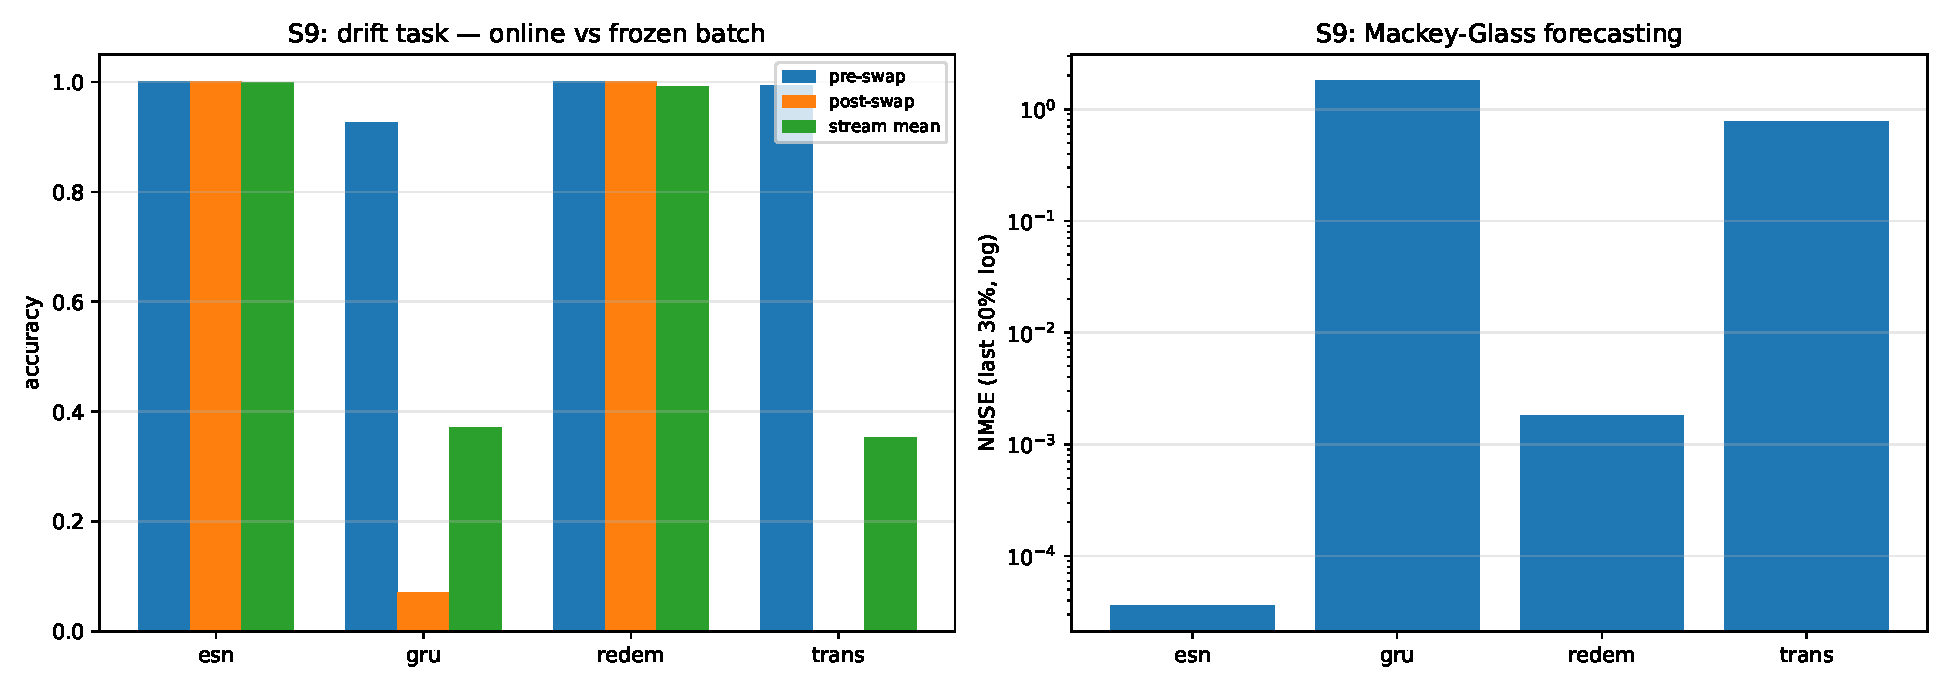
\includegraphics[width=0.85\textwidth]{paperB_fig6_showdown}
\caption{Baseline showdown: REDEM, matched online ESN, and
frozen GRU / tiny transformer on drift\_binary and Mackey--Glass.}
\label{fig:showdown}
\end{figure}

\begin{table}[t]
\centering
\caption{Standard-task comparison (10 seeds). REDEM and the ESN run online
with the same RLS readout; the ESN has 256 units with heterogeneous leak rates
matched to the $\tau$ distribution. The GRU and tiny transformer are frozen
batch models trained once on the first 30\% of the stream.}
\label{tab:bench}
\begin{tabular}{lcccc}
\toprule
Metric & REDEM & ESN & GRU & Transformer \\
\midrule
drift\_binary accuracy & 0.991 & 1.000 & 0.371 & 0.353 \\
Mackey--Glass NMSE     & 0.0018 & 0.000036 & 1.80 & 0.77 \\
\bottomrule
\end{tabular}
\end{table}

\textbf{Metadata transfer to the ESN.} To test whether the metadata mechanism
is substrate-specific, we gave the ESN the same slow EMA
state ($\tau_m = 500$, within the declared 200--1000-pulse range of
Eq.~\ref{eq:metadata}; unlike Section~\ref{sec:metadata}, which varies
$\tau_m\in\{200,1000\}$, the transfer experiment fixes a single value from
that range and performs no $\tau_m$ tuning) on the regime task. The result equalizes the systems:
ESN-with-metadata 0.998, ESN-fast 0.996, REDEM-full 0.994 (means over 10 seeds;
steady accuracy 1.000 for all; the REDEM-full arm here is an independent
re-run of the full system within this experiment's own 10-seed draw, not the
ablation run --- hence 0.994 vs.\ the 0.996 of
Section~\ref{sec:baselines}). Two conclusions follow. (i) The metadata is a
\emph{general, transferable} mechanism: it improves the ESN (0.996
$\rightarrow$ 0.998; boundary adaptation T40 49.9 $\rightarrow$ 40.6 pulses
with p90 76.5 $\rightarrow$ 42.0 under the switch-relative controlled
protocol) and REDEM (baseline
0.973 $\rightarrow$ full 0.994) alike --- the long-horizon statistical memory is
carried by the mechanism, not by any particular substrate. (ii) REDEM's
differentiation is therefore not raw accuracy on this task (where the ESN's
tanh reservoir with heterogeneous leak rates already partially covers the
regime statistics) but the surrounding mechanism set: the self-regulating
homeostat and structure plasticity that confer disturbance robustness
(Section~\ref{sec:homeo}), the local sparse coupling graph (the ESN is a dense
random reservoir with no self-regulation), and a timescale spectrum that is a
material property rather than a tuned hyperparameter.

\section{Discussion}
\label{sec:discussion}

\textbf{The architecture's niche.} REDEM occupies the online, fully-local
corner of the design space: it adapts to drift and disturbances that break
frozen batch models (which additionally require backpropagation through time),
and it adds substrate-level self-regulation --- a Lyapunov-estimating homeostat
and functional-connectivity rewiring --- that generic reservoirs lack. Against
a well-tuned ESN with the identical readout, REDEM is competitive on standard
tasks (drift accuracy 0.991 vs.\ 1.000; Mackey--Glass NMSE 0.0018 vs.\
$3.6\times10^{-5}$)
and superior on the dimensions the ESN lacks: disturbance robustness
(Section~\ref{sec:homeo}) and a locally coupled, physically motivated substrate
whose multi-timescale memory is set by material parameters rather than
hyperparameters. The metadata-transfer result (Section~\ref{sec:baselines})
shows that the long-horizon statistical mechanism is substrate-agnostic and
transfers its statistical-memory benefit to the ESN; disturbance-robustness
transfer does not hold (companion Paper~C~\cite{companionC}): recovery is the homeostat's
role, not the metadata's. REDEM's differentiation is the surrounding
mechanisms --- self-regulation, robustness, local coupling --- rather than
the metadata alone.

\textbf{Biological correspondence.} The three substrate-level mechanisms map
one-to-one onto established neural ideas: fast/slow memory (complementary
learning systems, hippocampus--cortex \cite{mcclelland1995}), homeostatic
regulation of excitability, and slow structural plasticity of connectivity ---
the correspondence taken at the level of local, activity-dependent plasticity
(as captured by spike-timing-dependent rules \cite{pfister2006}) rather than
of structural rewiring specifically. The
negative results sharpen the correspondence: reward signals without an error
channel fail exactly where predictive-coding theory says they should --- credit
assignment needs prediction error, and rewards only modulate.

\textbf{Limitations.} All results are numerical (Digital-Model level): the
substrate is a discrete relaxation model driven by deterministic
pseudo-random number generation and modeled on shallow-trap device physics,
with no hardware measurements or continuous-time cross-validation; the
physical claims are therefore design motivations to be validated on hardware,
not established physical facts. One seeding caveat concerns the frozen deep
baselines: their per-trial seeding (seed\_idx$\times$101$+$17) is applied
\emph{before} the GRU/transformer weight initialization, so each trial's
initialization is its own per-seed draw; the reported
baseline values are the values obtained by re-running the
script with this declared per-trial seeding. The task streams and the
substrate-driven arms
remain seeded and paired as declared in Section~\ref{sec:tasks}. The
single-disturbance robustness gains are
reproduced from the companion Paper~A rather than re-run here and cannot be
verified from this paper alone. The
readout-level comparison to the ESN is favorable to the ESN on standard
metrics; the metadata-transfer experiment shows the mechanism --- not the
substrate --- carries the long-horizon statistical memory, equalizing the
systems on the regime task (0.994--0.998); the substrate's differentiation
rests on its material-set memory design, the local sparse structure, and the
robustness mechanisms. The homeostat's task-level gains are masked by readout
compensation; the CPU-only scale ($N \le 1024$) leaves larger-scale behavior
untested.

\section{Conclusion}
\label{sec:conclusion}

REDEM demonstrates that a physically motivated relaxation substrate can host a
complete training-inference-unified learning system: an online error-driven
readout, a dual-timescale metadata memory, a chaos homeostat, and slow
structure plasticity, each validated individually and as an integrated system
that outperforms or ties every ablation and survives scale-up to $N=1024$.
A parameter sweep identifies the edge of chaos
($\lambda_{\mathrm{target}}{=}0$) as the best-supported homeostat target
($+25\%$ post-disturbance memory), although the integrated experiments
reported here were run at the earlier $\lambda_{\mathrm{target}}{=}-0.02$;
re-running them at the sweep optimum remains future work. The homeostat
maintains $+32\%$ memory capacity
after three sequential disturbances, and a causal audit confirms that all
adaptive mechanisms are causally clean at the operational leak magnitudes
tested. The two negative
results on reward-only learning fix the design boundary conditions: at the
readout an error channel is necessary; reward and intrinsic signals, being
structurally blind at the readout, are usable at the structure level
(Section~\ref{sec:homeo}). Honest benchmarking positions REDEM in the online/physical
niche: competitive with generic reservoirs on standard tasks, robust where
frozen batch learners fail, self-regulating under disturbance, and designed
for physical implementation --- with the long-horizon statistical mechanism shown to be
substrate-agnostic and transferable on statistical/streaming tasks
(disturbance robustness does not transfer with it \cite{companionC}).

\textbf{Future work.} A natural extension is to equip REDEM with a separate
long-term memory bank that periodically consolidates stable, repeatedly
encountered knowledge into the structural connectivity (M4), creating a
hierarchy between fast tracking and slow accumulation. This would address
stationary knowledge retention while preserving the system's responsiveness
to drift, but it would also introduce a consolidation-vs-overwrite trade-off
that lies beyond the scope of the present work. We leave this consolidation
mechanism to future investigation.

\section*{Declaration of competing interest}

The author declares no known competing financial interests or personal
relationships that could have appeared to influence the work reported in
this paper.

\section*{CRediT authorship contribution statement}

\textbf{Yaming Hu:} Conceptualization, Methodology, Software, Validation,
Formal analysis, Investigation, Data curation, Writing -- original draft,
Writing -- review \& editing, Visualization, Project administration.

\section*{Data availability}

All simulation data generated in this study are openly available at
\url{https://github.com/huyamingc/REDEM}.

\section*{Code availability}

All simulation scripts are openly available at
\url{https://github.com/huyamingc/REDEM}.

\section*{Funding}

This research did not receive any specific grant from funding agencies in
the public, commercial, or not-for-profit sectors.

\begin{thebibliography}{21}

\bibitem{parisi2019} Parisi, G. I., Kemker, R., Part, J. L., Kanan, C.,
Wermter, S. Continual lifelong learning with neural networks: a review.
\emph{Neural Networks} \textbf{113}, 54--71 (2019).

\bibitem{kirkpatrick2017} Kirkpatrick, J., Pascanu, R., Rabinowitz, N.,
Veness, J., Desjardins, G., Rusu, A. A., Milan, K., Quan, J., Ramalho, T.,
Grabska-Barwinska, A., Hassabis, D., Clopath, C., Kumaran, D., Hadsell, R.
Overcoming catastrophic forgetting in neural networks. \emph{Proceedings of
the National Academy of Sciences} \textbf{114}(13), 3521--3526 (2017).

\bibitem{sun2020} Sun, Y., Wang, X., Liu, Z., Miller, J., Efros, A., Hardt, M.
Test-time training with self-supervision for generalization under distribution
shifts. \emph{ICML} (2020).

\bibitem{rao1999} Rao, R. P. N., Ballard, D. H. Predictive coding in the visual
cortex: a functional interpretation of some extra-classical receptive-field
effects. \emph{Nature Neuroscience} \textbf{2}(1), 79--87 (1999).

\bibitem{friston2010} Friston, K. The free-energy principle: a unified brain
theory? \emph{Nature Reviews Neuroscience} \textbf{11}(2), 127--138 (2010).
\url{https://doi.org/10.1038/nrn2787}

\bibitem{strukov2008} Strukov, D. B., Snider, G. S., Stewart, D. R.,
Williams, R. S. The missing memristor found. \emph{Nature} \textbf{453}(7191),
80--83 (2008).

\bibitem{jaeger2001} Jaeger, H. The ``echo state'' approach to analysing and
training recurrent neural networks. GMD Report 148 (2001).

\bibitem{maass2002} Maass, W., Natschläger, T., Markram, H. Real-time computing
without stable states. \emph{Neural Computation} \textbf{14}(11), 2531--2560
(2002).

\bibitem{lukosevicius2009} Luko\v{s}evi\v{c}ius, M., Jaeger, H. Reservoir
computing approaches to recurrent neural network training. \emph{Computer
Science Review} \textbf{3}(3), 127--149 (2009).

\bibitem{haykin2002} Haykin, S. \emph{Adaptive Filter Theory}, 4th ed.
Prentice Hall (2002).

\bibitem{cho2014} Cho, K., van Merri\"enboer, B., Gulcehre, C., Bahdanau, D.,
Bougares, F., Schwenk, H., Bengio, Y. Learning phrase representations using
RNN encoder--decoder for statistical machine translation. \emph{Proceedings of
the 2014 Conference on Empirical Methods in Natural Language Processing
(EMNLP)}, 1724--1734 (2014).

\bibitem{vaswani2017} Vaswani, A., Shazeer, N., Parmar, N., Uszkoreit, J.,
Jones, L., Gomez, A. N., Kaiser, {\L}., Polosukhin, I. Attention is all you
need. \emph{Advances in Neural Information Processing Systems} \textbf{30},
5998--6008 (2017).

\bibitem{companionA} Author's companion Paper A: Memory and chaos in a
physics-constrained relaxation substrate: phase diagram, multi-timescale
forgetting, and disturbance robustness (substrate theory),
\emph{companion preprint} (2026),
\url{https://doi.org/10.5281/zenodo.22109664}.

\bibitem{benna2016} Benna, M. K., Fusi, S. Computational principles of synaptic
memory consolidation. \emph{Nature Neuroscience} \textbf{19}(12), 1697--1706
(2016).

\bibitem{fusi2005} Fusi, S., Drew, P. J., Abbott, L. F. Cascade models of
synaptically stored memories. \emph{Neuron} \textbf{45}(4), 599--611 (2005).

\bibitem{langton1990} Langton, C. G. Computation at the edge of chaos: phase
transitions and emergent computation. \emph{Physica D} \textbf{42}(1--3),
12--37 (1990).

\bibitem{bertschinger2004} Bertschinger, N., Natschläger, T. Real-time
computation at the edge of chaos in recurrent neural networks. \emph{Neural
Computation} \textbf{16}(7), 1413--1436 (2004).

\bibitem{hoerzel2014} Hoerzel, G., Legenstein, R., Maass, W. Emergence of
complex computational structures from chaotic neural networks through
reward-modulated Hebbian learning. \emph{Cerebral Cortex} \textbf{24}(3),
677--690 (2014).

\bibitem{companionC} Author's companion Paper C: Dissecting Online
Learning Mechanisms: Statistical Memory, Homeostatic Recovery, and
Substrate Physics are Non-Substitutable in the Directions and
Conditions Tested (three-mechanism disentanglement), \emph{companion
preprint} (2026),
\url{https://doi.org/10.5281/zenodo.22110618}.

\bibitem{mcclelland1995} McClelland, J. L., McNaughton, B. L., O'Reilly, R. C.
Why there are complementary learning systems in the hippocampus and neocortex.
\emph{Psychological Review} \textbf{102}(3), 419--457 (1995).

\bibitem{pfister2006} Pfister, J.-P., Gerstner, W. Triplets of spikes in a
model of spike timing-dependent plasticity. \emph{Journal of Neuroscience}
\textbf{26}(38), 9673--9682 (2006).
\url{https://doi.org/10.1523/JNEUROSCI.1425-06.2006}

\end{thebibliography}

\end{document}
